\subsection{The Cauchy-Schwarz and triangle inequalities}

The \textbf{Cauchy-Schwarz inequality}%
\index{Cauchy-Schwarz inequality!for dot product} is a fundamental
inequality satisfied by the dot product.  It is given in the following
proposition.

\begin{proposition}{Cauchy-Schwarz inequality}{cauchy-schwarz-inequality}
  The dot product satisfies the inequality
  \begin{equation}\label{cauchy}
    \abs{\vect{u}\dotprod \vect{v}}\leq \norm{\vect{u}} \norm{\vect{v}}
  \end{equation}
  Furthermore equality is obtained if and only if one of $\vect{u}$ or $\vect{v}$ is a scalar multiple of the other.
\end{proposition}

\begin{proof}
  First note that if $\vect{u}=\vect{0}$, then both sides of
  \eqref{cauchy} are equal to zero, and so the inequality holds in
  this case. Therefore, we will assume in what follows that
  $\vect{u}\neq \vect{0}$.  Define a function of $t\in \R$ by
  \begin{equation*}
    f(t) =(t\vect{u}+\vect{v}) \dotprod (t\vect{u}+ \vect{v}).
  \end{equation*}
  Then by Proposition~\ref{prop:properties-dot-product}, $f(t) \geq 0$
  for all $t\in \R$.  Also from
  Proposition~\ref{prop:properties-dot-product}, we have
  \begin{eqnarray*}
    f(t) &=&t\vect{u}\dotprod (t\vect{u}+\vect{v}) +
             \vect{v}\dotprod (t\vect{u}+\vect{v}) \\
         &=&t^2\vect{u}\dotprod \vect{u}+t(\vect{u}\dotprod \vect{v}) + t \vect{v}\dotprod \vect{u}+
             \vect{v}\dotprod \vect{v} \\
         &=&t^2\norm{\vect{u}}^{2}+2t(\vect{u}\dotprod \vect{v}) +\norm{
             \vect{v}} ^{2}.
  \end{eqnarray*}
  This means the graph of $y=f(t)$ is a parabola which opens upwards
  and is never negative. It follows that this function has at most one
  root. From the quadratic formula, we know that a quadratic function
  $at^2+bt+c$ has one or zero roots if and only if $b^2-4ac\leq
  0$. Applying this reasoning to the function $f(t)$, we obtain
  \begin{equation*}
    (2(\vect{u}\dotprod \vect{v})) ^{2}-4\norm{\vect{u}
    } ^{2}\norm{\vect{v}} ^{2}<0,
  \end{equation*}
  which is equivalent to
  $\abs{\vect{u}\dotprod \vect{v} }<\norm{\vect{u}} \norm{\vect{v}}$.
\end{proof}

An important consequence of the Cauchy-Schwarz inequality is the
so-called \textbf{triangle inequality}%
\index{triangle inequality!in Rn@in $\R^n$}, which states that the length
of one side of a triangle is less than or equal the sum of the lengths
of the two other sides.

\begin{proposition}{Triangle inequality}{triangle-inequality-dot-product}
  For\/ $\vect{u},\vect{v}\in \R^{n}$, we have
  \begin{equation}\label{triangle-ineq-1}
    \norm{\vect{u}+\vect{v}} \leq \norm{\vect{u}} +\norm{\vect{v}}.
  \end{equation}

  \begin{center}
    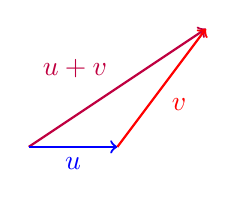
\begin{tikzpicture}[scale=1.5]
      \draw[->, thick, purple](0,0) -- node[above left]{$\vect{u}+\vect{v}$}(1.5,1);
      \draw[->, thick, blue](0,0) -- node[below]{$\vect{u}$} (0.75,0);
      \draw[->, thick, red](0.75,0) -- node[below right]{$\vect{v}$} (1.5,1);
    \end{tikzpicture}
  \end{center}
\end{proposition}

\begin{proof}
  By properties of the dot product and the Cauchy-Schwarz inequality,
  we have
  \begin{eqnarray*}
    \norm{\vect{u}+\vect{v}}^{2}
    &=& (\vect{u}+\vect{v})\dotprod(\vect{u}+\vect{v}) \\
    & =&(\vect{u}\dotprod\vect{u})+(\vect{u}\dotprod\vect{v})+(\vect{v}\dotprod\vect{u})+(\vect{v}\dotprod\vect{v}) \\
    &=&\norm{\vect{u}}^{2}+2(\vect{u}\dotprod\vect{v})+\norm{\vect{v}}^{2} \\
    &\leq& \norm{\vect{u}}^{2}+2\abs{\vect{u}\dotprod\vect{v}}+\norm{\vect{v}}^{2} \\
    &\leq& \norm{\vect{u}}^{2}+2\norm{\vect{u}}\norm{\vect{v}}+\norm{\vect{v}}^{2} \\
    &=& (\norm{\vect{u}}+\norm{\vect{v}})^{2}.
  \end{eqnarray*}
  Therefore,
  \begin{equation*}
    \norm{\vect{u}+\vect{v}}^{2}\leq(\norm{\vect{u}}+\norm{\vect{v}})^{2}.
  \end{equation*}
  Taking square roots of both sides, we obtain \eqref{triangle-ineq-1}.
\end{proof}

\begin{example}{Triangle inequality}{triangle-inequality}
  Use the triangle inequality to show
  \begin{equation*}
    \norm{\vect{u}} -\norm{\vect{v}} \leq \norm{\vect{u}-\vect{v}}
  \end{equation*}
  holds for all vectors $\vect{u},\vect{v}\in\R^n$.
\end{example}

\begin{solution}
  We have
  \begin{equation*}
    \norm{\vect{u}}
    = \norm{(\vect{u}-\vect{v})+\vect{v}} \\
    \leq \norm{\vect{u}-\vect{v}}+\norm{\vect{v}},
  \end{equation*}
  where we have used the triangle inequality in the last step. Note
  that this is an inequality between real numbers. Bringing
  $\norm{\vect{v}}$ to the other side of the equation, we have
  \begin{equation*}
    \norm{\vect{u}} - \norm{\vect{v}} \leq \norm{\vect{u}-\vect{v}}.
  \end{equation*}
\end{solution}
